\chapter{Experiments}
\label{chap:experiments}

All past chapters refer to the theory and name some theoretical implementation-details, all to verify the developed procedure.
However, this chapter presents some results to validate, that the spread of found paths really improves on maps of different scale.

\section{The testing-machine and simulation-setup}

    Firstly, the used machine runs an AMD Ryzen 7 3700X 8-Core Processor (\si{\num{3.6} \giga\hertz} base and \si{\num{4.4} \giga\hertz} max-boost) and has \si{\num{32} \giga\byte} of RAM built in, although only a few \si{\giga\byte} are needed (highly dependent on the map and number of threads).
    The operation-system is Arch Linux [x86\_64] with the kernel 5.7.9-arch1-1 installed.
    The used code for this thesis can be found in \cite{github:dominicparga/osmgraphing} and is implemented in Rust.
    Python is used for the visualization.
    Internally, this repository uses \cite{github:lesstat/multi-ch-constructor} (written in C++) as git-submodule for the \gls{contraction-hierarchies} and \cite{github:lesstat/nd-triangulation} for memory-management of the convex-hull.
    The latter is basically a Rust-wrapper for CGAL (C++).

    Graphs for street-networks are downloaded from \cite{osm}.
    Experiments run on the graph for Isle~of~Man (from March~2020) and on the graph for the German county Saarland (from July~2020).
    Considered \glspl{metric} are travel-distance (all paths tolerated) and travel-time (\si{40 \percent} tolerance on Isle~of~Man, \si{25 \percent} on Saarland).
    A tolerance of \si{25 \percent} refers to a worst-case-scenario of \si{15 \minute} more travel-time for originally \si{60 \minute}, which seems to be a good tradeoff.
    However, a tolerance of \si{40 \percent}, which is used for Isle~of~Man, refers to a worst-case of additional \si{24 \minute} for originally \si{60 \minute}.
    According to a simple Google-maps-query, one of the paths from one end of the island to the other takes $\approx \si{45 \minute}$.
    Hence, typical queries won't suffer that much.
    For routing, two sets of \num{10000}~\glspl{stpair} are chosen \gls{uar}\ from each map.
    One set is for \gls{balancing} on the particular map, the other set is for evaluating the balanced graph afterwards.
    This reduces the evaluation-results' dependence on the \gls{balancing}.
    Both sets are created in a way, such that a path can be found for every \gls{stpair} in the set.

    Two routing-algorithms, namely \gls{repr} on one side and \gls{dijkstra} with \gls{personalized_routing} on the other side, are used for the simulations.
    Due to \gls{balancing} and evaluation each use one routing-algorithm independent from each other, four simulation-scenarios occur:
    \begin{itemize}
        \item Both, \gls{balancing} and evaluating are done with \gls{dijkstra}.
            This scenario has the best performance of all scenarios, because \gls{repr} calls \gls{dijkstra} internally multiple times.
            On the other hand, \gls{repr} is already constructed to find a subset of pareto-optimal paths for same \glspl{stpair} and leads to a better spread.
            Most important, this case with using only \gls{dijkstra} doesn't guarantee a user-provided tolerance for found alternative paths.
            In general, \gls{dijkstra} finds the optimum path, but here, \gls{personalized_routing} is used.
            Hence, paths, that are optimal for some $\alpha$, can be arbitrary bad for a certain \gls{metric}, when compared to an optimal path of an $\alpha$ favoring only this \gls{metric} (\eg\ $(0, 1, 0, 0)^T$).
        \item Both \gls{balancing} and evaluating use \gls{repr}.
            This combination is expected to deliver the highest variety of alternative paths, but suffers from the highest runtime compared to simply running a \gls{dijkstra}-query.
            Besides that, \gls{repr} guarantees the user-provided tolerance for found paths due to its construction (see \vref{eq:new_init_alphas}).
        \item Two mixes of the previous cases are remaining, where \gls{balancing} is done with one routing-algorithm and evaluation with the other.
            Especially the case is interesting, where \gls{dijkstra} is used for \gls{balancing} and \gls{repr} for evaluation.
            The evaluation can be seen as representing a user-perspective.
            Hence, using \gls{dijkstra} with \gls{personalized_routing} for \gls{balancing} and \gls{repr} for evaluation keeps the guarantee for user-provided tolerances while keeping the \gls{balancing}-runtime reduced.
            As shown in the experiments, the results are not better than using only \gls{repr}, but still satisfactory.
    \end{itemize}

\todo{%
    TODO @Florian

    Verification: Does the product what it is specified for?

    Validation: Does the product solve the problem?
}

\section{Validating the simulation-results with Isle~of~Man}

    Isle~of~Man is a small island next to Great~Britain.
    The graph consists of around \num{50000}~nodes and \num{100000}~edges after parsing.
    The \gls{repr} uses a tolerance of \si{40 \percent} for travel-time and $\si{\num{99.8} \percent}$ of the graph's nodes are contracted.

    \subsection{Meta-data from balancing}
    \label{chap:experiments:meta}

        The simulation is not benchmarked in detail, but the coarse results in \vref{table:isle_of_man:balancing:performance} and \vref{table:isle_of_man:evaluating:performance} might help for getting an impression.
        Four threads are used.
        Please note, that the git-submodule for contracting graphs is rebuild in the first iteration without the new workload-\gls{metric} and build again in the following iteration with the new workload-\gls{metric} being considered.
        For Isle~of~Man, these build-times take much longer (still just $\si{\approx 1 \minute}$) than the actual contraction, for which reason below numbers discard the build-time.
        \begin{table}[htbp]
            \centering
            \begin{tabular}{ M{0.22\textwidth} || M{0.095\textwidth} M{0.095\textwidth} M{0.095\textwidth} || M{0.095\textwidth} M{0.095\textwidth} M{0.095\textwidth} }
                \multirow{2}{*}{Isle~of~Man} & \multicolumn{3}{c ||}{Balanced with \gls{dijkstra}} & \multicolumn{3}{c}{Balanced with \gls{repr}} \\
                & Iteration 0 & Iteration 1 & Iteration 2 & Iteration 0 & Iteration 1 & Iteration 2 \\
                \hline
                \hline
                Average query-time before contraction & $\approx \si{7 \milli\second}$ & $\approx \si{7 \milli\second}$ & $\approx \si{7 \milli\second}$ & $\approx \si{7 \milli\second}$ & $\approx \si{7 \milli\second}$ & $\approx \si{7 \milli\second}$ \\
                \hline
                Time for contracting ($\si{\num{99.8} \percent}$ of $|V|$) & $\approx \si{5 \second}$ & $\approx \si{5 \second}$ & $\approx \si{5 \second}$ & $\approx \si{5 \second}$ & $\approx \si{5 \second}$ & $\approx \si{5 \second}$ \\
                \hline
                Average speed-up through contraction & $\infty$ & $\infty$ & $\infty$ & $\infty$ & $\infty$ & $\infty$ \\
                \hline
                Time for balancing & $\approx \si{1 \second}$ & $\approx \si{1 \second}$ & $\approx \si{1 \second}$ & $\approx \si{2 \second}$ & $\approx \si{25 \second}$ & $\approx \si{30 \second}$ \\
                \hline
                Number of found paths ($\mu \pm \sigma$) & $1 \pm 0$ & $1 \pm 0$ & $1 \pm 0$ & $\approx 3 \pm 2$ & $\approx 15 \pm 24$ & $\approx 19 \pm 24$ \\
                \hline
                Maximum workload & \num{891} & \num{1620} & \num{783} & \num{852} & \num{795} & \num{722} \\
                \hline
                Number of unique edges (in \num{1000}) & $\approx \num{82.1}$ & $\approx \num{81.7}$ & $\approx \num{82.2}$ & $\approx \num{82.8}$ & $\approx \num{84.2}$ & $\approx \num{83.9}$ \\
            \end{tabular}
            \caption[Overview of performance when balancing Isle~of~Man]{%
                Isle~of~Man.
                An overview (but no detailled benchmarks) of \gls{balancing}-performance with four threads on Isle~of~Man.
                Here, $\si{\num{99.8} \percent}$ of all nodes are contracted.
                In \cref{table:isle_of_man:evaluating:performance} describing the performance during evaluation, the graph isn't contracted to show the contraction's impact on performance.
                The query-times before contraction refer to \gls{dijkstra}-queries from the contraction-tool, so are independent of the \gls{balancing}'s routing-algorithm.
                The maximum workloads are just copied from the plots.
                The number of found paths ($\ge 1$) is provided with a standard-deviation to indicate, that the mean is not caused by some outliers.
                The number of unique edges stands for the actual number of edges in $|E|$ with a workload greater than zero.
                The set of \glspl{stpair} contains \num{10000}~\glspl{stpair}.
                \label{table:isle_of_man:balancing:performance}
            }
        \end{table}

        \todo{%
            TODO @Florian

            Approval with statement about standard-deviation below? Nice!?
        }
        Besides a first impression of the needed runtime, \vref{table:isle_of_man:balancing:performance} already explains the differences in performance.
        The needed time for the \gls{balancing}, basically just path-searches, is much smaller with \gls{dijkstra} than with \gls{repr}, because \gls{repr} calls \gls{dijkstra} multiple times.
        The number of found paths increases with iteration-number when using \gls{repr}, which is desirable.
        Because the standard-deviations are greater than the respective means (and the number of found paths is at least one for every \gls{stpair} due to selection of \glspl{stpair}), any small number of found paths requires a high number (or several respective high numbers) on the other side of the mean.
        This indicates, that the means are probably not caused just by some outliers.
        Further, the number of covered edges in $|E|$ is higher after \gls{balancing} and improves more with \gls{repr} than with \gls{dijkstra}.

    \subsection{Actual results from balancing}

        The \gls{balancing} consists of two workload-\gls{metric}-updates, but all together, workload-plots of three iterations can be found on the following pages.
        Every workload leads to a new \gls{metric}-update, but the last iteration doesn't update the workload-\gls{metric}, so the last workloads show the final spread of paths over the street-network, after the final workload-\gls{metric}-update is adapted.
        Despite randomness and different sets of \glspl{stpair}, these final workloads should be identical to those from evaluation in \cref{chap:experiments:isle_of_man:eval}.
        The workloads in \cref{fig:isle_of_man/dijkstra/0/workloads} and \vref{fig:isle_of_man/repr/0/workloads} lead to the first \gls{metric}-update.
        In fact, due to construction (see \vref{eq:averaging}), the first workloads are the actual new workload-\gls{metric} after the update (after normalization by their mean).

        \begin{figure}[hbp]
            \centering%
            %
            \subfloat[%
                Initial workloads with \gls{dijkstra}
            ]{%
                \includegraphics[width=0.49\textwidth]{isle_of_man/balanced_with_dijkstra/0/workloads}\label{fig:isle_of_man/dijkstra/0/workloads}
            }%
            \hfill%
            \subfloat[%
                Workloads after first update with \gls{dijkstra}
            ]{%
                \includegraphics[width=0.49\textwidth]{isle_of_man/balanced_with_dijkstra/1/workloads}\label{fig:isle_of_man/dijkstra/1/workloads}
            }%

            \subfloat[%
                Initial workloads with \gls{repr}
            ]{%
                \includegraphics[width=0.49\textwidth]{isle_of_man/balanced_with_repr/0/workloads}\label{fig:isle_of_man/repr/0/workloads}
            }
            \hfill%
            \subfloat[%
                Workloads after first update with \gls{repr}
            ]{%
                \includegraphics[width=0.49\textwidth]{isle_of_man/balanced_with_repr/1/workloads}\label{fig:isle_of_man/repr/1/workloads}
            }%
            \caption[Initial workloads and bad first iteration when balancing Isle~of~Man]{%
                Isle~of~Man.
                The first row shows the balancing with \gls{dijkstra}, the second row shows the balancing with \gls{repr}.

                The left side is showing the workloads in the first iteration, right before the first workload-\gls{metric}-update.
                Thus, only the existing \glspl{metric} are used for routing.

                The right side is showing the workloads after the first and in the second iteration, right before the final workload-\gls{metric}-update.
                \Gls{dijkstra} has a much worse maximum workload, but all color-bars are kept identical.
                \label{fig:isle_of_man/both/0/workloads}
                \label{fig:isle_of_man/both/1/workloads}
            }
        \end{figure}

        The initial plots \cref{fig:isle_of_man/dijkstra/0/workloads} and \cref{fig:isle_of_man/repr/0/workloads} are quite identical.
        This is not an issue of \gls{repr}, but of the considered \glspl{metric}.
        Both, travel-distance and travel-time, don't bring that different paths without any artificial \gls{metric}.
        Although, some more paths occur on the graph showing workloads from \gls{repr}, leading to an insignificantly smaller maximum workload here.

        The plots of the second iteration, which is the first iteration including an artificial \gls{metric}, can be seen in \cref{fig:isle_of_man/dijkstra/1/workloads} and \vref{fig:isle_of_man/repr/1/workloads}.
        As mentioned in \cref{chap:balancing:update}, the first update doesn't lead to a spreaded workload yet.
        Especially \gls{dijkstra} results in a maximum workload, that is twice as high as before.
        Nonetheless, in \cref{fig:isle_of_man/dijkstra/1/workloads} (after first update \gls{balancing} with \gls{dijkstra}), there are still some new found routes in between (\eg\ in the north of the map).
        In this second iteration, the previously updated workload-\gls{metric} makes \gls{dijkstra} avoid popular routes more or less completely.
        But on such a small map, quite many of these popular routes use the fastest streets in the street-network.
        The same holds for \gls{repr}, but \gls{repr} does still consider the tolerance of $\si{40 \percent}$, thus the found paths tend to stick with previously found routes, as you can see in \cref{fig:isle_of_man/repr/1/workloads}.
        The maximum workload of paths from \gls{repr} is slightly better than in the initial iteration.
        Even some more spread is visible in \cref{fig:isle_of_man/repr/1/workloads}.
        However, despite some exceptions, the spread is still quite identical to the initial one, when compared to the globally best spreaded workloads after \gls{balancing}, shown in \vref{fig:isle_of_man/both/2/workloads}.

        \begin{figure}[hbp]
            \centering%
            %
            \subfloat[%
                Initial workloads with \gls{dijkstra}
            ]{%
                \includegraphics[width=0.49\textwidth]{isle_of_man/balanced_with_dijkstra/0/workloads}
            }%
            \hfill%
            \subfloat[%
                After second and last update with \gls{dijkstra}
            ]{%
                \includegraphics[width=0.49\textwidth]{isle_of_man/balanced_with_dijkstra/2/workloads}\label{fig:isle_of_man/dijkstra/2/workloads}
            }%

            \subfloat[%
                Initial workloads with \gls{repr}
            ]{%
                \includegraphics[width=0.49\textwidth]{isle_of_man/balanced_with_repr/0/workloads}
            }
            \hfill%
            \subfloat[%
                After second and last update with \gls{repr}
            ]{%
                \includegraphics[width=0.49\textwidth]{isle_of_man/balanced_with_repr/2/workloads}\label{fig:isle_of_man/repr/2/workloads}
            }%
            \caption[Workloads during balancing Isle~of~Man in comparison]{%
                Isle~of~Man.
                These plots show the workloads during \gls{balancing}.
                The graph is balanced with \gls{dijkstra} and \gls{repr}.
                The first row shows the \gls{balancing} with \gls{dijkstra}, whereas the second row shows the \gls{balancing} with \gls{repr}.
                The left side shows the workloads before the first workload-\gls{metric}-update, whereas the right side shows the workloads after two workload-\gls{metric}-updates.
                Furthermore, despite randomness and the different \glspl{stpair} from evaluation, the plots on the right side correspond to the evaluation-plots in \vref{fig:isle_of_man/both/both/1/workloads}.
                The used \glspl{metric} besides the new workload-\gls{metric} are travel-distance and travel-time.
                When using \gls{repr}, each path's travel-time tolerates a maximum of \si{\num{40} \percent} worse than its optimum.
                \label{fig:isle_of_man/both/2/workloads}
            }
        \end{figure}

        With the final workloads after \gls{balancing} with \gls{repr}, shown in \vref{fig:isle_of_man/repr/2/workloads}, it is noticable, how the clear hotspots from the initial plots flew into multiple new paths in between.
        At the same time, these hotspots don't vanish at all, so most popular paths are still popular, while the overall situation improved.
        This is good, because most popular means more optimal with respect to travel-time.
        In opposite to that, after \gls{balancing} with \gls{dijkstra}, shown in \cref{fig:isle_of_man/dijkstra/2/workloads}, the workload looks less distributed than in \cref{fig:isle_of_man/repr/2/workloads} (final workload after \gls{balancing} with \gls{repr}).
        This doesn't necessarily imply, that the graph's balance is that much worse.
        In fact, when evaluating the \gls{dijkstra}-balanced graph with \gls{repr} (see \vref{fig:isle_of_man/dijkstra/repr/1/workloads}), the resulting workloads actually look more spreaded than the final workloads from \gls{balancing} with \gls{dijkstra} (see \cref{fig:isle_of_man/dijkstra/2/workloads}), noticable by the different colors in the middle of the respective plots.
        A comparison of the number of found paths confirms on that in \vref{table:isle_of_man:evaluating:performance} (evaluating-performance).

        Lastly, \cref{chap:balancing} claims and explains, that two iterations are intuitively a good choice, because popular and alternative routes are balanced here.
        Running Isle~of~Man for more than two iterations supports this statement.
        The relevant information about the iterations are provided in \vref{table:isle_of_man/repr/10/workloads}.
        After the second \gls{metric}-update, the maximum-workloads are worse or equal (slightly better here and there) and number of unique edges are quite similar.
        But most important, the number of found paths is much worse than before, so indeed less paths are found with more iterations.
        Besides that, the \gls{balancing} takes, of course, much more time with more iterations, while the workloads after two and after ten \gls{metric}-updates (see \vref{fig:isle_of_man/repr/10/workloads}) are more or less identical.

        \begin{figure}[hbp]
            \centering%
            %
            \subfloat[%
                After second \gls{metric}-update with \gls{repr}
            ]{%
                \includegraphics[width=0.49\textwidth]{isle_of_man/balanced_with_repr/2/workloads}
            }%
            \hfill%
            \subfloat[%
                After tenth \gls{metric}-update with \gls{repr}
            ]{%
                \includegraphics[width=0.49\textwidth]{isle_of_man/balanced_with_repr/10/workloads}\label{fig:isle_of_man/repr/10/workloads}
            }%
            \caption[Comparison of two and ten metric-updates when balancing Isle~of~Man]{%
                Isle~of~Man.
                These plots show the workloads during \gls{balancing}.
                The graph is balanced with \gls{repr}.
                The left plot shows the workloads after two \gls{metric}-updates, whereas the right plot shows the workloads after ten \gls{metric}-updates.
                The plots are more or less identical, but \cref{table:isle_of_man/repr/10/workloads} shows clear differences.
                The used \glspl{metric} besides the new workload-\gls{metric} are travel-distance and travel-time.
                When using \gls{repr}, each path's travel-time tolerates a maximum of \si{\num{40} \percent} worse than its optimum.
            }
        \end{figure}

        \begin{table}[htbp]
            \centering
            \begin{tabular}{ M{0.21\textwidth} || M{0.096\textwidth} | M{0.096\textwidth} M{0.096\textwidth} M{0.096\textwidth} M{0.096\textwidth} M{0.096\textwidth} }
                \multirow{2}{*}{Isle~of~Man} & \multicolumn{6}{c}{Balanced with \gls{repr}} \\
                & Iteration 2 & Iteration 3 & Iteration 4 & Iteration 5 & Iteration 6 & Iteration 7 \\
                \hline
                \hline
                Number of found paths ($\mu \pm \sigma$) & $\approx 19 \pm 24$ & $13 \pm 18$ & $\approx 13 \pm 17$ & $\approx 15 \pm 20$ & $14 \pm 16$ & $\approx 15 \pm 19$ \\
                \hline
                Maximum workload & \num{722} & \num{789} & \num{746} & \num{729} & \num{760} & \num{712} \\
                \hline
                Number of unique edges (in \num{1000}) & $\approx \num{83.9}$ & $\approx \num{84.1}$ & $\approx \num{84.1}$ & $\approx \num{84.0}$ & $\approx \num{84.1}$ & $\approx \num{83.8}$ \\
                \multicolumn{7}{c}{} \\
                & Iteration 2 & Iteration 8 & Iteration 9 & Iteration 10 & & \\
                \hline
                \hline
                Number of found paths ($\mu \pm \sigma$) & $19 \pm 24$ & $14 \pm 18$ & $\approx 15 \pm 19$ & $\approx 16 \pm 22$ & & \\
                \hline
                Maximum workload & \num{722} & \num{838} & \num{710} & \num{796} & & \\
                \hline
                Number of unique edges (in \num{1000}) & $\approx \num{83.9}$ & $\approx \num{83.9}$ & $\approx \num{83.9}$ & $\approx \num{83.9}$ & &
            \end{tabular}
            \caption[Comparison of two and ten metric-updates when balancing Isle~of~Man]{%
                Isle~of~Man.
                A comparison of iterations to show, that two \gls{metric}-updates are indeed a good choice.
                Here, iteration 2 refers to the respective iteration 2 in \cref{table:isle_of_man:balancing:performance}.
                The number of found paths ($\ge 1$) is provided with a standard-deviation to indicate, that the mean is not caused by some outliers.
                The number of unique edges stands for the actual number of edges in $|E|$ with a workload greater than zero.
                \label{table:isle_of_man/repr/10/workloads}
            }
        \end{table}

    \subsection{Comparison of evaluating different scenarios}
    \label{chap:experiments:isle_of_man:eval}

        The evaluation is basically recreating the workloads from last \gls{balancing}-iteration with switching routing-algorithms and another set of \glspl{stpair}.
        So paths for all \glspl{stpair} are searched and the street-network's workload is counted again, which is shown in the evaluation-related plots in the following.
        A new set of \num{10000}~\glspl{stpair} is determined, again chosen \gls{uar},\ to reduce the evaluation-results' dependence on the \gls{balancing}.

        In \vref{table:isle_of_man:evaluating:performance} (evaluation-related performance), similar information as in \vref{table:isle_of_man:balancing:performance} (\gls{balancing}-related performance) is noted (and relevant parts are copied).
        To show the huge performance-impact of using \gls{contraction-hierarchies}, the evaluation is done without contracting the balanced graph.
        The initial number of unique edges with the new set for \gls{dijkstra} is $\approx \num{82000}$, for \gls{repr} it is $\approx \num{82800}$.
        Besides the performance, especially the average number of found paths is interesting.
        When \gls{balancing} and evaluating with \gls{repr}, the average number of found paths is $\approx 19 \pm 25$.
        Evaluating with \gls{repr}, but \gls{balancing} with \gls{dijkstra} still brings out $\approx 12 \pm 17$ paths on average.
        Note, that the actual number of found paths is at least one due to selection of \glspl{stpair}, and that the meaning of the standard-deviation is explained in \cref{chap:experiments:meta}.
        These two means show, that doing \gls{balancing} with \gls{dijkstra} is quite good, and confirm, that the similar looking initial workloads from \gls{balancing} (in \vref{fig:isle_of_man/both/0/workloads}) and the initial workloads from evaluating (in \vref{fig:isle_of_man/both/both/0/workloads}) are indeed an issue of the \glspl{metric}, not of \gls{repr}.

        \begin{table}[htbp]
            \centering
            \begin{tabular}{ M{0.21\textwidth} || M{0.096\textwidth} | M{0.096\textwidth} M{0.096\textwidth} || M{0.096\textwidth} | M{0.096\textwidth} M{0.096\textwidth} }
                \multirow{2}{*}{Isle~of~Man} & \multicolumn{3}{c ||}{Balanced with \gls{dijkstra}} & \multicolumn{3}{c}{Balanced with \gls{repr}} \\
                & Iteration & \multicolumn{2}{c ||}{Evaluated with} & Iteration & \multicolumn{2}{c}{Evaluated with} \\
                & 2 & \gls{dijkstra} & \gls{repr} & 2 & \gls{dijkstra} & \gls{repr} \\
                \hline
                \hline
                Time for searching all paths & $\approx \si{1 \second}$ & $\approx \si{13 \second}$ & $\approx \si{8 \minute}$ & $\approx \si{30 \second}$ & $\approx \si{12 \second}$ & $\approx \si{14 \minute}$ \\
                \hline
                Number of found paths ($\mu \pm \sigma$) & $1 \pm 0$ & $1 \pm 0$ & $\approx 12 \pm 17$ & $\approx 18$ & $1 \pm 0$ & $\approx 19 \pm 25$ \\
                \hline
                Maximum workload & \num{783} & \num{789} & \num{786} & \num{722} & \num{689} & \num{750} \\
                \hline
                Number of unique edges (in \num{1000}) & $\approx \num{82.2}$ & $\approx \num{82.1}$ & $\approx \num{83.9}$ & $\approx \num{83.9}$ & $\approx \num{82.4}$ & $\approx \num{83.9}$ \\
            \end{tabular}
            \caption[Comparison of performance between balancing (contracted) and evaluating (not contracted) Isle~of~Man]{%
                Isle~of~Man.
                A comparison (but no detailled benchmarks) of evaluating-performance with the \gls{balancing}-performance (from \vref{table:isle_of_man:balancing:performance}), using again four threads on Isle~of~Man.
                Here, iteration 2 refers to the respective iteration 2 in \cref{table:isle_of_man:balancing:performance}.
                This time, when evaluating, the graph isn't contracted (for comparison) and hence the runtime is much longer.
                The number of found paths ($\ge 1$) is provided with a standard-deviation to indicate, that the mean is not caused by some outliers.
                The number of unique edges stands for the actual number of edges in $|E|$ with a workload greater than zero.
                The initial number of unique edges with the new evaluation-set (also \num{10000}~\glspl{stpair}) for \gls{dijkstra} is $\approx \num{82000}$, for \gls{repr} it is $\approx \num{82800}$.
                \label{table:isle_of_man:evaluating:performance}
            }
        \end{table}

        The workloads, that are generated by ignoring the new workload-\gls{metric} and that use the new evaluation-set of \glspl{stpair}, are shown in \vref{fig:isle_of_man/both/both/0/workloads}.
        They are looking more or less identical to the initial workloads from \gls{balancing} in \vref{fig:isle_of_man/both/0/workloads}, but are still provided for completeness.
        Additionally, \cref{fig:isle_of_man/both/both/1/delta_workloads} shows the differences between evaluated workloads without and with the new workload-\gls{metric}.
        Only the differences of \gls{balancing} and evaluting \gls{dijkstra} and \gls{balancing} and evaluting \gls{repr} are presented, to show the most extreme distinctions.
        Both plots reduce the workload on previously popular routes and increase the workload on less popular routes.
        However, the \gls{repr}-plot showing the workload differences through evaluating (in \cref{fig:isle_of_man/repr/repr/1/delta_workloads}) contains more spots for little increases than the respective \gls{dijkstra}-plot (in \cref{fig:isle_of_man/dijkstra/dijkstra/1/delta_workloads}) does, which concentrates more on the previously popular streets.
        This consolidates in the maximum changes, which are clearly higher (around $\pm 600$) for \gls{dijkstra} than for \gls{repr} (around $\pm 400$).

        \begin{figure}[hbp]
            \centering%
            %
            \subfloat[%
                Initial workloads with \gls{dijkstra}
            ]{%
                \includegraphics[width=0.49\textwidth]{isle_of_man/balanced_with_dijkstra/evaluation/with_dijkstra/0/workloads}\label{fig:isle_of_man/dijkstra/dijkstra/0/workloads}
            }%
            \hfill%
            \subfloat[%
                Difference between initial workloads (left) and final workloads (\cref{fig:isle_of_man/dijkstra/dijkstra/1/workloads}) using \gls{dijkstra} for both \gls{balancing} and evaluating
            ]{%
                \includegraphics[width=0.49\textwidth]{isle_of_man/balanced_with_dijkstra/evaluation/with_dijkstra/1/delta_workloads}\label{fig:isle_of_man/dijkstra/dijkstra/1/delta_workloads}
            }%

            \subfloat[%
                Initial workloads with \gls{repr}
            ]{%
                \includegraphics[width=0.49\textwidth]{isle_of_man/balanced_with_repr/evaluation/with_repr/0/workloads}\label{fig:isle_of_man/repr/repr/0/workloads}
            }%
            \hfill%
            \subfloat[%
                Difference between initial workloads (left) and final workloads (\cref{fig:isle_of_man/repr/repr/1/workloads}) using \gls{repr} for both \gls{balancing} and evaluating
            ]{%
                \includegraphics[width=0.49\textwidth]{isle_of_man/balanced_with_repr/evaluation/with_repr/1/delta_workloads}\label{fig:isle_of_man/repr/repr/1/delta_workloads}
            }%
            \caption[Initial workloads and workload-changes when evaluating balanced Isle~of~Man]{%
                Isle~of~Man.
                These plots show the balanced graph evaluated with \gls{dijkstra} and \gls{repr}.
                The first row shows the evaluation with \gls{dijkstra} after \gls{balancing} with \gls{dijkstra}, whereas the second row shows the evaluation with \gls{repr} after \gls{balancing} with \gls{repr}.
                The left side shows the evaluation without the new workload-\gls{metric}.
                These plots look quite identical to \vref{fig:isle_of_man/both/0/workloads} (initial plots of \gls{balancing}), but since the evaluation uses a different set of \glspl{stpair}, it is needed for the sake of completeness.
                The right side shows the workload-changes from the initial workloads here to the respective \cref{fig:isle_of_man/dijkstra/dijkstra/1/workloads} and \cref{fig:isle_of_man/repr/repr/1/workloads}.
                The used \glspl{metric} are travel-distance and travel-time, and additionally the new workload-\gls{metric} for the differences.
                When using \gls{repr}, each path's travel-time tolerates a maximum of \si{\num{40} \percent} worse than its optimum.
                \label{fig:isle_of_man/both/both/0/workloads}
                \label{fig:isle_of_man/both/both/1/delta_workloads}
            }
        \end{figure}

        The probably most interesting plots are depicted in \vref{fig:isle_of_man/both/both/1/workloads}.
        Note, that the previous plots from \vref{fig:isle_of_man/both/2/workloads} (showing the \gls{balancing}'s last iterations' workloads) are the same cases than the evaluation-related plots in \cref{fig:isle_of_man/dijkstra/dijkstra/1/workloads} and \cref{fig:isle_of_man/repr/repr/1/workloads}, just with a different set of \glspl{stpair}.
        Both plots, that show the workloads of the balanced graph evaluated, are clearly more spreaded than the initial evaluation-plots from \cref{fig:isle_of_man/both/both/0/workloads}, because the maximum workloads are lower and the most popular routes are flown into other routes according to the color-shifts in the plots.
        Just using \gls{dijkstra} (\cref{fig:isle_of_man/dijkstra/dijkstra/1/workloads}) still seems to be tradeoff towards performance, because popular routes are basically just moved to another place.
        On the other hand, using \gls{dijkstra} for queries after \gls{balancing} with \gls{repr} surprisingly reduces the maximum workload the most.
        Especially in the north of the map, this combination (\cref{fig:isle_of_man/repr/dijkstra/1/workloads}) shows a few more routes than using just \gls{dijkstra} (\cref{fig:isle_of_man/dijkstra/dijkstra/1/workloads}).
        Still an issue, when using \gls{dijkstra} with \gls{personalized_routing}, is the not guaranteed tolerance for found paths' cost.
        That's why the most important combinations are those, where \gls{repr} is used as evaluation-query (or user-query respectively), because these two combinations consider the optimum path with respect to travel-time.
        Both \gls{balancing} with \gls{dijkstra} (\cref{fig:isle_of_man/dijkstra/repr/1/workloads}) and \gls{balancing} with \gls{repr} (\cref{fig:isle_of_man/repr/repr/1/workloads}) show more distribution in the middle of the map, noticable at respectively colored spots (\eg\ around longitude of \num{-4.6}).
        Though, only using \gls{repr} clearly delivers the best spreaded results, again noticable by more reduced workloads overall, but at a much higher performance-cost during \gls{balancing}.

        \begin{figure}[hbp]
            \centering%
            %
            \subfloat[%
                Balanced and evaluated with \gls{dijkstra}
            ]{%
                \includegraphics[width=0.49\textwidth]{isle_of_man/balanced_with_dijkstra/evaluation/with_dijkstra/1/workloads}\label{fig:isle_of_man/dijkstra/dijkstra/1/workloads}
            }%
            \hfill%
            \subfloat[%
                Balanced with \gls{dijkstra} and evaluated with \gls{repr}
            ]{%
                \includegraphics[width=0.49\textwidth]{isle_of_man/balanced_with_dijkstra/evaluation/with_repr/1/workloads}\label{fig:isle_of_man/dijkstra/repr/1/workloads}
            }%

            \subfloat[%
                Balanced with \gls{repr} and evaluated with \gls{dijkstra}
            ]{%
                \includegraphics[width=0.49\textwidth]{isle_of_man/balanced_with_repr/evaluation/with_dijkstra/1/workloads}\label{fig:isle_of_man/repr/dijkstra/1/workloads}
            }%
            \hfill%
            \subfloat[%
                Balanced and evaluated with \gls{repr}
            ]{%
                \includegraphics[width=0.49\textwidth]{isle_of_man/balanced_with_repr/evaluation/with_repr/1/workloads}\label{fig:isle_of_man/repr/repr/1/workloads}
            }%
            \caption[Workloads on the balanced graph of Isle~of~Man]{%
                Isle~of~Man.
                These plots show the balanced graph evaluated with \gls{dijkstra} and \gls{repr}.
                The first row shows the evaluation after \gls{balancing} with \gls{dijkstra}, whereas the second row shows the evaluation after \gls{balancing} with \gls{repr}.
                The left side shows the evaluation with \gls{dijkstra}, whereas the right side shows the evaluation with \gls{repr}.
                The used \glspl{metric} besides the new workload-\gls{metric} are travel-distance and travel-time.
                When using \gls{repr}, each path's travel-time tolerates a maximum of \si{\num{40} \percent} worse than its optimum.
                \label{fig:isle_of_man/both/both/1/workloads}
            }
        \end{figure}

    \section{Additional validation with Saarland}

        Saarland is a small German county.
        The graph consists of around \num{580000}~nodes and \num{1160000}~edges after parsing, which is around ten times larger than Isle~of~Man.
        The \gls{repr} uses a tolerance of \si{25 \percent} for travel-time (in contrary to $\si{40 \percent}$ with Isle~of~Man) and also $\si{\num{99.8} \percent}$ of the graph's nodes are contracted.

        With Isle~of~Man, every aspect is talked about, but trying out a larger map has revealed the lack of convergence with the first Euler-approach (see \cref{eq:euler}) and lead to the second and working averaging-approach (see \cref{eq:averaging}).
        Therefore, it is helpful and necessary to run larger maps, for which reason Saarland is also presented shortly in the following.
        Besides that, the new plots show some new behaviour on less loaded maps.

        First of, the \gls{balancing}-performance is shown in \vref{table:saarland:balancing:performance} and the evaluating-performance (contracted this time) in \vref{table:saarland:evaluating:performance}, similar to Isle~of~Man before.
        As described earlier, but with much more impact in a larger map, is the performance-advantage of \gls{dijkstra} over \gls{repr}.
        Doing the whole \gls{balancing} with \gls{dijkstra} takes a few minutes, while using \gls{repr} a little more than an hour.
        The reason is clear, since \gls{repr} does find much more alternative paths, which are all not worse than $\si{\num{25} \percent}$ of the optimum path with respect to travel-time.
        This opens the question to reduce the tolerance (\eg\ $\si{\num{20} \percent}$ or even $\si{\num{15} \percent}$).
        Much more remarkable is the number of found paths from the evaluation-performance (\cref{table:saarland:evaluating:performance}) for \gls{balancing} with \gls{dijkstra} and evaluating (executing user-queries) with \gls{repr}.
        This combination finds even more alternative paths than using just \gls{repr}.

        When looking at the evaluation-plots in \vref{fig:saarland/both/both/1/workloads}, it is obvious, that the \gls{dijkstra}-plots (\cref{fig:saarland/dijkstra/dijkstra/1/workloads} and \cref{fig:saarland/repr/dijkstra/1/workloads}) have much lower maximum-workload (under \num{500}) than the \gls{repr}-plots (more than \num{700}), what can be seen in the final \gls{balancing}-plot of \gls{dijkstra} (\cref{fig:saarland/dijkstra/2/workloads}) as well.
        Here should be noted, that \gls{dijkstra} doesn't consider the tolerance at all and such a barely loaded street-network offers plenty of space to spread.
        However, the two results using \gls{repr} for evaluation-queries (or user-queries respectively) are quite identical, whereas \gls{balancing} with \gls{dijkstra} (\cref{fig:saarland/dijkstra/repr/1/workloads}) needs a fraction of the runtime of \gls{balancing} with \gls{repr} (\cref{fig:saarland/repr/repr/1/workloads}).
        Even similar improvements and new routes can be seen on both plots, especially between longitude of \num{7.0} and \num{7.2} around the latitude of \num{49.35}.
        So, in addition to Isle~of~Man, using \gls{dijkstra} for \gls{balancing} and \gls{repr} for user-queries seems to be a good compromise.

        \begin{table}[htbp]
            \centering
            \begin{tabular}{ M{0.21\textwidth} || M{0.0985\textwidth} M{0.0985\textwidth} M{0.0985\textwidth} || M{0.0985\textwidth} M{0.0985\textwidth} M{0.0985\textwidth} }
                \multirow{2}{*}{Saarland} & \multicolumn{3}{c ||}{Balanced with \gls{dijkstra}} & \multicolumn{3}{c}{Balanced with \gls{repr}} \\
                & Iteration 0 & Iteration 1 & Iteration 2 & Iteration 0 & Iteration 1 & Iteration 2 \\
                \hline
                \hline
                Average query-time before contraction & $\approx \si{115 \milli\second}$ & $\approx \si{130 \milli\second}$ & $\approx \si{125 \milli\second}$ & $\approx \si{124 \milli\second}$ & $\approx \si{120 \milli\second}$ & $\approx \si{121 \milli\second}$ \\
                \hline
                Time for contracting ($\si{\num{99.8} \percent}$ of $|V|$) & $< \si{30 \second}$ & $\approx \si{1 \minute}$ & $\approx \si{1 \minute}$ & $< \si{30 \second}$ & $\approx \si{1 \minute}$ & $\approx \si{1 \minute}$ \\
                \hline
                Average speed-up through contraction & $\approx \num{135}$ & $\approx \num{144}$ & $\approx \num{37}$ & $\approx \num{136}$ & $\approx \num{36}$ & $\approx \num{34}$ \\
                \hline
                Time for balancing & $\approx \si{22 \second}$ & $\approx \si{24 \second}$ & $\approx \si{25 \second}$ & $\approx \si{5 \minute}$ & $\approx \si{21 \minute}$ & $\approx \si{47 \minute}$ \\
                \hline
                Number of found paths ($\mu \pm \sigma$) & $1 \pm 0$ & $1 \pm 0$ & $1 \pm 0$ & $6 \pm 3$ & $12 \pm 25$ & $28 \pm 33$ \\
                \hline
                Maximum workload & \num{725} & \num{658} & \num{442} & \num{914} & \num{971} & \num{774} \\
                \hline
                Number of unique edges (in \num{1000}) & $\approx \num{474}$ & $\approx \num{509}$ & $\approx \num{481}$ & $\approx \num{488}$ & $\approx \num{493}$ & $\approx \num{502}$ \\
            \end{tabular}
            \caption[Overview of performance when balancing Saarland]{%
                Saarland.
                An overview (but no detailled benchmarks) of \gls{balancing}-performance with 15 threads on Saarland.
                Here, also $\si{\num{99.8} \percent}$ of all nodes are contracted.
                The query-times before contraction refer to \gls{dijkstra}-queries from the contraction-tool, so independent of the \gls{balancing}'s routing-algorithm.
                The maximum workloads are just copied from the plots.
                The number of found paths ($\ge 1$) is provided with a standard-deviation to indicate, that the mean is not caused by some outliers.
                The number of unique edges stands for the actual number of edges in $|E|$ with a workload greater than zero.
                The set of \glspl{stpair} contains \num{10000}~\glspl{stpair}.
                \label{table:saarland:balancing:performance}
            }
        \end{table}

        \begin{table}[htbp]
            \centering
            \begin{tabular}{ M{0.21\textwidth} || M{0.096\textwidth} | M{0.096\textwidth} M{0.096\textwidth} || M{0.096\textwidth} | M{0.096\textwidth} M{0.096\textwidth} }
                \multirow{2}{*}{Saarland} & \multicolumn{3}{c ||}{Balanced with \gls{dijkstra}} & \multicolumn{3}{c}{Balanced with \gls{repr}} \\
                & Iteration & \multicolumn{2}{c ||}{Evaluated with} & Iteration & \multicolumn{2}{c}{Evaluated with} \\
                & 2 & \gls{dijkstra} & \gls{repr} & 2 & \gls{dijkstra} & \gls{repr} \\
                \hline
                \hline
                Time for searching all paths & $\approx \si{25 \second}$ & $< \si{2 \minute}$ & $\approx \si{54 \minute}$ & $\approx \si{47 \minute}$ & $\approx \si{28 \second}$ & $\approx \si{47 \minute}$ \\
                \hline
                Number of found paths ($\mu \pm \sigma$) & $1 \pm 0$ & $1 \pm 0$ & $\approx 32 \pm 36$ & $\approx 28 \pm 33$ & $1 \pm 0$ & $\approx 28 \pm 33$ \\
                \hline
                Maximum workload & \num{442} & \num{485} & \num{770} & \num{774} & \num{469} & \num{789} \\
                \hline
                Number of unique edges (in \num{1000}) & $\approx \num{481}$ & $\approx \num{479}$ & $\approx \num{501}$ & $\approx \num{502}$ & $\approx \num{487}$ & $\approx \num{502}$ \\
            \end{tabular}
            \caption[Comparison of performance between balancing and evaluating Saarland]{%
                Saarland.
                A comparison (but no detailled benchmarks) of evaluating-performance with the \gls{balancing}-performance (from \vref{table:saarland:balancing:performance}), using again 15 threads on Saarland.
                Here, iteration 2 refers to the respective iteration 2 in \cref{table:saarland:balancing:performance}.
                This time, when evaluating, the graph is contracted (in opposite to previously with Isle~of~Man).
                The number of found paths ($\ge 1$) is provided with a standard-deviation to indicate, that the mean is not caused by some outliers.
                The number of unique edges stands for the actual number of edges in $|E|$ with a workload greater than zero.
                The initial number of unique edges with the new evaluation-set (also \num{10000}~\glspl{stpair}) for \gls{dijkstra} is $\approx \num{471000}$, for \gls{repr} it is $\approx \num{487000}$.
                \label{table:saarland:evaluating:performance}
            }
        \end{table}

        \begin{figure}[hbp]
            \centering%
            %
            \subfloat[%
                Initial workloads with \gls{dijkstra}
            ]{%
                \includegraphics[width=0.49\textwidth]{saarland/balanced_with_dijkstra/0/workloads}\label{fig:saarland/dijkstra/0/workloads}
            }%
            \hfill%
            \subfloat[%
                After second and last update with \gls{dijkstra}
            ]{%
                \includegraphics[width=0.49\textwidth]{saarland/balanced_with_dijkstra/2/workloads}\label{fig:saarland/dijkstra/2/workloads}
            }%

            \subfloat[%
                Initial workloads with \gls{repr}
            ]{%
                \includegraphics[width=0.49\textwidth]{saarland/balanced_with_repr/0/workloads}\label{fig:saarland/repr/0/workloads}
            }
            \hfill%
            \subfloat[%
                After second and last update with \gls{repr}
            ]{%
                \includegraphics[width=0.49\textwidth]{saarland/balanced_with_repr/2/workloads}\label{fig:saarland/repr/2/workloads}
            }%
            \caption[Workloads on the balanced graph of Saarland]{%
                Saarland.
                These plots show the workloads during \gls{balancing}.
                The graph is balanced with \gls{dijkstra} and \gls{repr}.
                The first row shows the \gls{balancing} with \gls{dijkstra}, whereas the second row shows the \gls{balancing} with \gls{repr}.
                The left side shows the workloads before the first workload-\gls{metric}-update, whereas the right side shows the workloads after two workload-\gls{metric}-updates.
                Furthermore, despite randomness and the different \glspl{stpair} from evaluation, the plots on the right side correspond to the evaluation-plots in \vref{fig:saarland/both/both/1/workloads}.
                The used \glspl{metric} besides the new workload-\gls{metric} are travel-distance and travel-time.
                When using \gls{repr}, each path's travel-time tolerates a maximum of \si{\num{25} \percent} worse than its optimum.
                \label{fig:saarland/both/0/workloads}
                \label{fig:saarland/both/2/workloads}
            }
        \end{figure}

        \begin{figure}[hbp]
            \centering%
            %
            \subfloat[%
                Balanced and evaluated with \gls{dijkstra}
            ]{%
                \includegraphics[width=0.49\textwidth]{saarland/balanced_with_dijkstra/evaluation/with_dijkstra/1/workloads}\label{fig:saarland/dijkstra/dijkstra/1/workloads}
            }%
            \hfill%
            \subfloat[%
                Balanced with \gls{dijkstra} and evaluated with \gls{repr}
            ]{%
                \includegraphics[width=0.49\textwidth]{saarland/balanced_with_dijkstra/evaluation/with_repr/1/workloads}\label{fig:saarland/dijkstra/repr/1/workloads}
            }%

            \subfloat[%
                Balanced with \gls{repr} and evaluated with \gls{dijkstra}
            ]{%
                \includegraphics[width=0.49\textwidth]{saarland/balanced_with_repr/evaluation/with_dijkstra/1/workloads}\label{fig:saarland/repr/dijkstra/1/workloads}
            }%
            \hfill%
            \subfloat[%
                Balanced and evaluated with \gls{repr}
            ]{%
                \includegraphics[width=0.49\textwidth]{saarland/balanced_with_repr/evaluation/with_repr/1/workloads}\label{fig:saarland/repr/repr/1/workloads}
            }%
            \caption[Workloads on the balanced graph of Saarland]{%
                Saarland.
                These plots show the balanced graph evaluated with \gls{dijkstra} and \gls{repr}.
                The first row shows the evaluation after \gls{balancing} with \gls{dijkstra}, whereas the second row shows the evaluation after \gls{balancing} with \gls{repr}.
                The left side shows the evaluation with \gls{dijkstra}, whereas the right side shows the evaluation with \gls{repr}.
                The used \glspl{metric} besides the new workload-\gls{metric} are travel-distance and travel-time.
                When using \gls{repr}, each path's travel-time tolerates a maximum of \si{\num{25} \percent} worse than its optimum.
                \label{fig:saarland/both/both/1/workloads}
            }
        \end{figure}